\chapter{Metoder}
Metode kapitlet beskriver projektets arbejdsmetoder, hvilke metoder der brugt og hvordan de er blevet brugt. Metodeafsnittet vil især beskrive projektstyringsforløb og udviklingsmetoderne. 

\section{Projektstyring} \label{title:projektstyring}
Til overordnet projektstyring er der gjort brug af den \textit{Struktureret Agile Metode}, forkortet SAM. (Se hjemmeside \fixme{Reference til http://www.agilemanifesto.org/iso/dk/}). Metoden karakteriseres ved at inddele projektet i følgende faser: krav, design, implementering og test. Metoden passede godt på projektet i flere omstændigheder. SAM er oplagt til projektgrupper i størrelsen 2-3 personer og projekter der varer 3-9 måneder. Metoden er også særlig anvendelig til projektet da inddragelse af kunden fylder en stor del i arbejdet. 
Især i arbejde med forprojektet og opstartsfasen på projektet blev der afholdt mange møder for at fastlægge projektets rammer og kravene til produktet. I SAM metoden adskiller man møder i forskellige kategorier og de tre kategori er som følger: \textit{introduktionsmøde, planlægningsmøde og kontraktmøde}. Samarbejdet med kunde Rolf Blauenfeldt kan meget vel inddeles i tre forskellige møde kategorier. I forprojektet afholdte projektgruppen \textit{introduktionsmøde} med kunden for at forventningsafstemme. Da det var på plads og projektgruppen havde besluttet at kundens problemstilling var en opgave som gruppen kunne løse, blev der afholdt flere \textit{planlægningsmøder} for at finde og udspecificere de  krav som kunden havde til produktet. Disse møder er afholdt over flere omgange, da der undervejs i projekt er opstået situationer, som ikke var blevet fastlagte. Men efter der var afholdt tilstrækkeligt \textit{planlægningsmøder} igangsatte projektgruppen første fase af SAM metoden og der blev udarbejdet en kravspecifikation(Se afsnit \ref{title:kravspecifikation}). SAM faserne er iterative processer, derfor blev der undervejs i forløbet  foretaget ændringer og justeringer i kravspecifikationen. Kort efterfulgt af kravspecifikation er der udarbejdet en accepttest (Se afsnit \ref{title:accepttest}), som blev udfyldt da udviklingen af prototypen var færdig. Inden arbejdet med prototypen begyndte, blev der udarbejdet et system design (Se afsnit \ref{title:systemdesign}), for at fastlægge hvordan systemet skulle struktureres. Da system strukturen var fastlagt begyndt implementeringsfasen og slutter med at gennemføre accepttesten. For uddybende information se afsnit \ref{title:udviklingMetode} omkring udviklingsdokumentationen.

\subsection{Scrum/Pivotaltracker} \label{title:scrum}
Til arbejdsfordeling og planlægning af arbejdsopgaver er projektet udarbejdet ved hjælp af scrum. Der er ikke brugt scrum i direkte forstand. Men hver uge er blevet set som et sprint, hvor der hver mandag er udarbejdet en sprint backlog som skulle udføres i ugens løb. Emnerne til sprint backlogen er bla. taget fra tidsplanen som kan ses som en overordnet projekt backlog. Sidst på ugen er der afholdt møde, hvor der opsamles på ugens arbejdet og hvilke opgaver i sprint backloggen der er blevet løst. Opgaver, der ikke blev løst, er automatisk blevet videreført til næste uges backlog. Hver mandag når der oprettes et sprint backlog er disse opgaver blevet oprettet i projektstyringsværktøjet \textit{pivotaltracker} ( se hjemmeside \fixme{https://www.pivotaltracker.com/}). Ca. halvvejs inde i projektet blev det besluttet at arbejdsbyrden ved anvendelse af pivotaltracker var alt for stor, sammenlignet med det ekstra overblik over scrum det gav. Pivotaltracker er et godt redskab til større grupper, men på grund projektgruppens størrelse er ugentlige og daglige korte morgenmøder langt mere effektivt. Overblik over scrum anvendt i dette projekt kan ses på figur \ref{fig:scrumProcess}

	\begin{figure}[H]
		\centering
		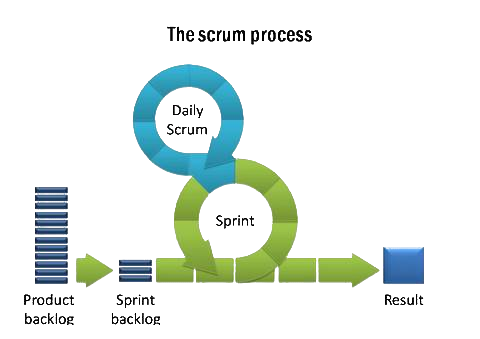
\includegraphics[width = 0.6\textwidth]{billeder/scrumProcess.png}
		\caption{Scrum model. Produkt backloggen indeholder alle de opgave, som dette projekt består af. Springt backloggen indeholder de opgaver som det ugentlige sprint tager opgaver fra. Et sprint gennemføres i dette projekt på ugentligt basis. sprintets indhold er bestemt i de to ugentlige møder mandag og fredag (se ugeplan og logbog \ref{title:ugeplanOgLogbog}). Det daglige scrum er styret af morgenmødet. Resultatet er \textit{konditioneringsapparatet} med alt tilhørende dokumentation}\label{fig:scrumProcess}
	\end{figure}
\fixme{ref: https://presentation-process-img.s3.amazonaws.com/SCRUM\%20POWERPOINT/scrum-process.JPG    Dato: 3-12-2015}

\subsection{Samarbejdsaftale}
For at sikre interne forventninger til projektarbejde i gruppen, har gruppens medlemmer lavet og underskrevet en samarbejdsaftale i begyndelse af projektet. Aftalen kan læses i \ref{title:samarbejdsaftaleIntern}.

I forbindelse med samarbejdet med reviewgruppen, er der også blevet udarbejdet og underskrevet en samarbejdsaftale, for at sikre ens forventning til reviewmøderne. Aftalen kan læses i \ref{title:samarbejdsaftaleReview}.

\subsection{Samarbejdspartnere} \label{title:samarbejdspartnere}
Dette afsnit beskriver projektgruppens samarbejdspartnere igennem projektet. 

\textbf{Kunden og projektudbyder:} Rolf Ankerlund Blauenfeldt er læge ved neurologisk afsnit på Aarhus Universitet (AUH). Samarbejdet med Rolf har primært bestået i specificering af krav til udvikling af \textit{Konditioneringsapparatet} samt faglig ekspert for remote ischemic conditioning (RIC). Desuden er det kunden som godkender accepttesten.

\textbf{Vejleder:} Projektvejleder Peter Johansen, har været som faglig vejleder i gennem hele projektet og igennem vejledermøder Peter bistået med faglig kritik løbende. 

\textbf{Reviewgruppe:} Igennem projektet er der samarbejdet med en anden projektgruppe, hhv. Anders Esager og Anders Toft. Denne gruppe har fungeret som opponent/review gruppe, og hver gang en milepæl var nået, fx accepttest, har grupperne reviewet hinandens opgaver, hvorefter et møde er blevet afholdet og rettelserne er blevet gennemgået.  

\textbf{Firma:} Virksomheden Seagul forhandler blodtryksapparater og har i projektets opstart fungeret som kontaktperson til en kinesisks udviklingsvirksomhed. Samarbejdet blev oprettet for at projektgruppen kunne modtage teknisk sparring i specifikations- og udviklingsfasen. 

\textbf{Advokat:} I forbindelse med tavshedspligt (Se afsnit \ref{title:tavshedspligt}) har projektgruppen samarbejdet med juridisk rådgiver Maibrit Lerche Hendriksen fra Aarhus Universitet. Pga. projektgruppen ønskede samarbejde med en reviewgruppe, kunne samarbejdet ikke begynde før reviewgruppen også blev underlagt tavshedspligt.

\subsubsection{Medikoteknisk afd. AUH}
Til udvikling og kalibrering af \textit{Konditioneringsapparatet} har projektgruppen samarbejdet med medikotekniske ingeniører  Sara Rose Newell og Steven Brantlov fra Region Midtjylland. Disse har kunne bistå med en blodtrykssimulator, samt teknisk forståelse af blodtryksmåling. Samarbejdet har bestået i mail korrespondance, samt to møder på medikoteknisk afsnit på AUH, hvor projektgruppen har testet og kalibreret \textit{Konditioneringsapparatet} på blodtrykssimulatoren. 

\subsubsection{Lungemedicinsk afsnit og Troels Johansen}
I forbindelse med udvikling af sikkerhedskontrol til konditioneringsapparatet(Se afsnit \ref{title:sikkerhedskontrol} omkring projektafgrænsninger) har projektgruppen samarbejdet med Troels Johansen, PhD studerende ved lungemedicinsk afdelingen på AUH. Samarbejdet opstod pga. gruppen manglede ekspertviden omkring pulsoximeteri og afklemning.

\subsubsection{Institut for idræt og Kristian Vissing} 
Efter okklusionstræning blev en del prototypens funktionalitet, havde projektgruppen behov for mere indsigt omkring træningsformen. Her blev etableret et samarbejde med Kristian Vissing, lektor og forsker ved Institut for Idræt, Aarhus Universitet.  

\subsection{Ugeplan og logbog}
Som del af projektstyring, udviklingsproces, samt dagbog, er der på ugentlig basis udarbejdet en plan. Hver uge starter med en ugeplan og afsluttes med en logbog. Ugeplanen indholder de opgaver projektgruppen skal løse i ugens løb og logbogen er en opsamling på ugens arbejde. For uden at fungere som sprint backlog i scrum (Se afsnit \ref{title:scrum}) har logbogen også fungeret som en slags dagbog, hvor projekts forløb konstant er blevet beskrevet. Logbogen har også været særlig anvendeligt forbindelse med rapport skrivning. 

\subsection{Vejldermøde}
Fra projektets opstart blev der aftalt et vejledermøde i alle ulige uger under projektforløbet. Disse møder er blevet brugt til at sikre at projektarbejdet hele tiden var på rette spor, samt faglig vejledning til projektarbejdet. Desuden er vejledermøderne brugt til at få konstruktiv feedback på færdige dokumenter undervejs i forløbet. 

\subsection{Tidsplan}
I forbindelse med forprojektet blev der udarbejdet en tidsplan i gantt chart format (se afsnit \ref{title:tidsplan}). Et gantt chart illutreret start og slut dato for hvert af projektet delelementer. Hver række i tidsplanen udgør et delelement, fx. kravspecifikation og accepttesten og hver kolonne udgør én uge. Tidsplanen er løbende blevet opdateret efterhånden som projekt har nået delelementerne. 

\subsection{Tavshedspligt} \label{title:tavshedspligt}
Pga. af patentundersøgelse har hele projekt været underlagt tavshedspligt og underskrevet tavshedserklæringer med både universitet og neurologisk afsnit. Tavshedspligten har bla. forsinket nogle processer da alle parter skulle have underskrevet en tavshedserklæring inden. I andre tilfælde hvor et samarbejde har været kortvarig eller der ikke har været tid til at underskrive tavshedserklæring, har projektgruppen måtte undlade detaljer ved kommunikation med disse samarbejdspartnere. Dette har i nogle tilfælde betydet at hjælpen fra evt. eksperter har været begrænset af manglende forståelse for projektet.  Derfor har den igangværende patentundersøgelse været et begrænsning for projektarbejdet i flere omfang. \fixme{Reference til tavshedserklæring}
Tavshedspligten har også betydet at der skulle tages bestemte hensyn i forbindelse med versionsstyring. Ved brug af git (Se afsnit \ref{title:versionsstyring} omkring versionsstyring) som versionsstyrings værktøj, har gruppen skulle betale for at få et private repository. Dette er normal gratis, men så er ens repository offentligt tilgængeligt. 


\section{Versionsstyring} \label{title:versionsstyring}
For at sikre korrekt og brugervenlig versionsstyring af hele projektets versionsstyring blevet håndteret med git \fixme{Reference til git hjemmeside https://github.com/}. Git er versionsstyring primært udviklet til software. Styringen af versionshistorik fungere ved at der oprettes et respository, som ligger på en ekstern server. Hver gang der ønskes at arbejde på filerne i det oprettede repository, skal der synkroniseres, så den seneste version er tilgængelig. Foretages en ændring i en fil der køres versionshistorik på, skal denne \textit{committes} til ens repository. Alle ændringer der tilføjes, skal beskrives, for at sikre sporbarhed. Resten af versionsstyring foregår automatisk i git, og her gemmes automatisk versionsnummer og dato for ændring. Desuden gør git det også nemt at gå tilbage i versionshistorikken og finde tidligere versioner. 
Selvom prototypen \textit{Konditioneringsapparatet} ikke skal medicinsk godkendes, var det en grund til at vælge et detaljeret versionsstyrings system. Hvis et apparat skal medicinsk godkendelse stilles der store krav til dokumentationen, heriblandt versionsstyring, som indgår i kvalitetssikringen af produktet (Se afsnit \ref{title:medGodkendelse} ). 
Til grafisk interface findes en række programmer som gør git og versionsstyring mere brugervenligt, og her har det især været brugbart at kunne se forrige ændringer og tilføjelse. Dette har lettet projektarbejdet og mindsket uoverensstemmelser med hvilket dokument der er af seneste version. 

Udover git er dropbox brugt til at dele projektfiler, der ikke har behov for versionsstyring. Dette har fx. været videnskabelige artikler, datablade mm. 

\section{Udviklingsværktøjer}\label{title:udviklingsvaerktoejer}
\textbf{Eclipse:} er blevet brugt til software udvikling af \textit{Konditioneringsapparatet}. For at kunne simplificere kommunikation mellem eclipse og arduino boardet, er der blevet brugt et arduino plugin i eclipse. På den måde kan funktionaliteterne fra Arduino IDE bruges, samtidig med at eclipse funktionaliteter, som \textit{auto complete}, fejlhåndtering og projektstruktur også var tilstedet. 

\textbf{Arduino IDE:} er den oprindelig udviklingsplatform til arduino, men pga af manglende funktionalitet, er dette kun blevet brugt til simple enhedstests og små scripts. 

\textbf{Matlab:} Til databehandling og visualisering af signaler fra \textit{Konditioneringsapparatet}. Værktøjet er blevet brugt til at plotte tryk kurver fra tryksensoren, samt oscillationerne målt fra manchetten. Dette har været en stor hjælp for signal forståelse og i forbindelse med kalibrering af blodtryksmåleren. 

\textbf{Fritzing:} er blevet brugt til udarbejdning af fumlebræt tegning og schematics over hardware udvikling. Grundet prototype udviklingen har meget af arbejdet foregået på fumlebræt, og for at kunne dokumentere og "gemme" en opsætning på fumlebrættet har \textit{fritzing} været stor hjælp til bla. fejlhåndtering. \textit{Fritzing} er et open source program som er udviklet til dokumentation af prototyper. Da programmet er open source har processen med at finde nye komponenter været simpel. 

\textbf{Gimp:} Billede redigerings program som er blevet brugt til redigering og udarbejdelse af illustrationer. Især i forbindelse med figurer og illustrationer til latex har gimp været anvendeligt. 

\textbf{Maple:} Til filter udregning i forbindelse med design af analoge og digitale filtre er der blevet brugt Maple version 2015. Maple er kommercielt computer algebra system. 

\textbf{Modelio:} Alt udvikling af sysML og UML er foregået i Modelio. Modelio adskiller sig fra andre sysML værktøjer, da det ikke er et tegne program, men et programmeringssprog og IDE. Dette betyder at udviklingen af sysML har været begrænset af sproget, men det betyder også at det har været nemmere at overholde sysML standarden. 

\textbf{TexStudio:} Alt dokumentation er blevet udarbejdet i TexStudio. Dette er valgt for at få fuld kontrol over layoutet i dokumentationen og rapporten. LaTeX og TeXStudio gør også arbejdet med større projekter mere simpel, ved opdeling af dokumentationen i små underdokumenter.


\section{Udviklingsproces} \label{title:udviklingMetode}
Efter den struktureret agil metodes(SAM) fire faser: krav, design, implementering og test (se afsnit \ref{title:projektstyring}) er udviklingsprocessen foregået i denne rækkefølge. Disse fire faser vil blive beskrevet nedenfor.

	\subsection{Kravspecifikation} \label{title:kravspecifikation}
	Kravspecifikation er et dokument der beskriver de krav som produktet skal kunne. Der skelnes mellem funktionelle og ikke funktionelle krav. De funktionelle krav beskriver de essentielle krav for at produktet kan leve op til kundens behov. Et eksempel på et funktionelt krav er at apparatet skal kunne afklemme med tryk på 25 mmHg over det systoliske blodtryk. I kravspecifikation er de funktionelle krav beskrevet via \textit{fully dressed use cases}. En use case beskriver brugen med produktet i scenarier og ved hjælp af disse scenarier beskrives produktets funktionalitet. En \textit{fully dressed use case} indeholder, ud over en beskrivelse af hoved scenariet, også beskrivelse af hvilke aktører der er involveret i scenariet, samt før og efter betingelse for scenariet. I nogle scenarier kan det også være nødvendigt at beskrive undtagelser for forløbet, hvis disse ikke er for trivielle. Aktørerne der indgår i \textit{fully dressed use cases} er beskrevet med en aktørbeskrivelse i kravspecifikation. Her beskrives aktør rollen, og om han er primær eller sekundær. En primær aktør interagerer aktivt med produktet i use casen og er nødvendig for at scenariet lykkes. En sekundær aktør er passivt involveret med use casen og dette kan for eksempel være en patient der skal modtage behandling med et apparat. For at give læseren et overblik over sammenhængen mellem aktører og use cases, indeholder kravspecifikation et overordnet use case diagram, hvor alle scenerier er listet og aktørernes rolle er beskrevet med pile forbundet med use cases. 
	
	De ikke-funktionelle krav, er som navnet antyder, krav der ikke er nødvendige for produktets funktionalitet. Ikke-funktionelle krav er essentielle for brugervenligheden, sikkerheden og muligheden for at vedligeholde produktet. Ved specifikations af de ikke-funktionelle krav, indskærpes rammerne for udviklingen af produktet. Et eksempel på et funktionelt krav er at produktet skal kunne gemme information omkring konditioneringsbehandlingen på et SD kort. Her kan stilles et ikke-funktionelt krav, der specificeret datastrukturen på SD kortet og hvilken type SD produktet skal kunne håndtere. Det sikre brugervenlighed og sikkerhed, fordi brugeren ved hvordan data gemmes og hvilke SD kort der kan bruges i produktet. Herved imødekommes eventuelle data tab ved forkerte SD kort. For at fastlægge rammerne for udseende af prototypen, indeholder kravspecifikationen også illustrationer af bruger interfacet. 
	
	\subsection{Accepttest} \label{title:accepttest}
	Accepttest er en metode og en del af udviklingsprocessen, som er udarbejdet for at produktet kan leve op til kravspecifikation. Accepttesten er essentielt for produktudviklingen, for den udføres og godkendes i samarbejdet med kunden. Når accepttesten er gennemført er det kundens endegyldige godkendelse af produktet. 
	Dokumentet er struktureret med en tabel for hver use case, denne tabel indeholder punkterne fra hoved scenariet og hvert punkt indeholder en beskrivelse, en test metode, et forventet resultat og til sidste et felt hvor testen kan godkendes. Det samme struktur gælder for de ikke funktionelle krav. Hver test skal godkendes med underskrift af kunden.
	
	\subsection{System design} \label{title:systemdesign}
	Dette trin i udviklingsprocessen vedrører designet af \textit{Konditioneringsapparatet}. For at sikre overensstemmelse inden udviklingsprocessen blev igangsat, blev systemets design og arkitektur beskrevet. System designet indeholder først en beskrivelse af alle systemets underdele. Her beskrivelses hvilke dele der skal indgå i systemet for at det lever op til designet.
	For at sikre at alle områder i systemet designet blev belyst er der her gjort brug af metoden \textit{4 plus 1 modellen} på figur \ref{fig:4plus1model}. Modellen er oprindelig kun beregnet til software men i dette projekt er den tilpasset og bruges på systemet som helhed. 
	
	\begin{figure}[H]
		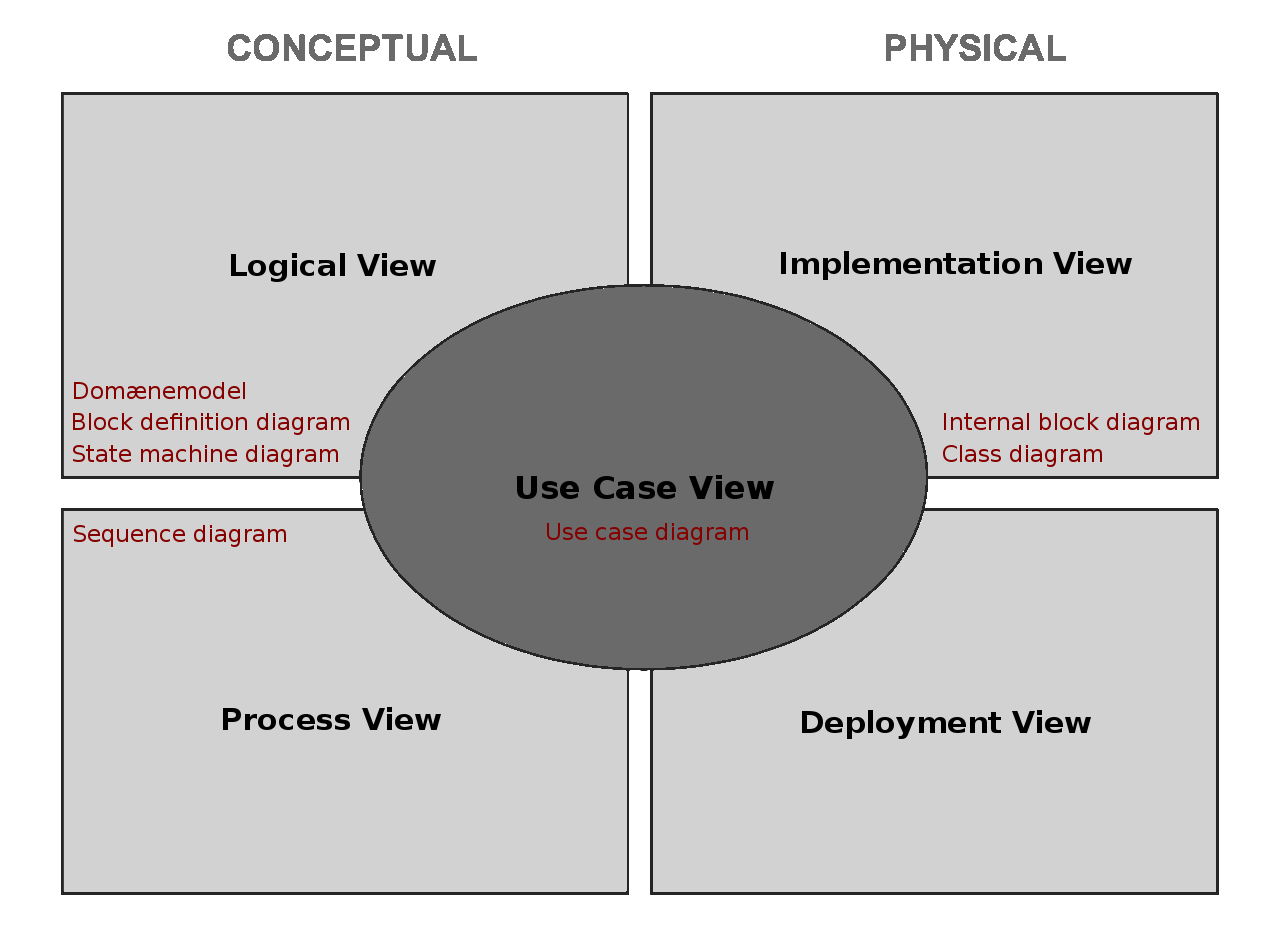
\includegraphics[width = \textwidth]{billeder/4plus1model.png}
		\caption{Tilpasset 4 + 1 model. Den røde tekst er de diagramtyper fra UML, som hører til de 5 inddelinger og er anvendt i dette projekt.}\label{4plus1model}
	\end{figure}
	
	4+1 modellen ser produktet fra fire forskellige synsvinkler og sikre at alle partners interesser er belyst. De fire synsvinker er som følger: 
	\\ \textit{Use case view}: Beskriver systemmet med aktører og de forskellige senarier de interagerer i. Dette er beskrevet i kravspecifikationen se (\fixme{ref: kravspec}).\\
	\textit{Logical view}: Denne synsvinkel beskriver systemets funktionalitet via centrale elementer, mekanismer og stadier. Synsvinklen er generelt mere abstrakt end de andre 3. \\
	\textit{Process view}: Beskæftiger sig med de dynamiske aspekter af systemet, forklaring system processer, hvordan de kommunikerer og fokuserer på systemets opførsel i drift. \\
	\textit{Implementation view}: Denne vinkel involverer udviklerens perspektiv og beskæftiger sig med hvordan software implementeres. \\
	\textit{Deployment view:} Beskriver systemet fra en fysisk synsvinkel, blandt andet hvordan eksekveringen af softwares skal foregå på apparatet og hvordan systemets fysisk setup skal ser ud. \\
	\textit{NB: Beskrivelse af de fire synsvinkler er udklip fra system design dokumentet.} \fixme{Indsæt reference til system design}
	
	I system design dokumentet er der også gjort stor brug af sysML diagram sproget. Sproget er universel blandt ingeniører og letter forståelsen af systemet. I \textit{Logical view} er der udarbejdet state machine diagrammer, som bruges til at beskrive stadierne som produktet kan befinde sig i, samt hvordan der skiftes mellem disse stadier. I \textit{process view} fokuseres der på hvordan systemet dele interagerer med hinanden. Til at beskrive denne kommunikation bruges sekvens diagrammer. Der er udarbejdet et sekvens diagram for hver use case. Sekvensdiagrammer beskriver hvordan scenarieret fra use case udføres i mellem systemets dele, samt hvilken information der videregives mellem underdelene. 
	
	\subsection{Implemetering} \label{title:implementering}
	Implementeringen af produktets funktionalitet er beskrevet i implementeringsdokumentet. Dette dokument bruges til at beskrive hvordan systemets enkelte software og hardware dele er implementeret og hvordan disse underdele har opnået deres ønskede funktionalitet. Dokumentet har også til formål at fungere som et opslagsværk, så ønsker læseren forståelse for en specifik software eller hardware del, står det i implementeringsdokumentet. Derfor skal implementeringsdokumentet også ses som en \textit{opskrift} på hvordan produktet er fremstillet. Dokumentet indeholder især erfaringer omkring arbejdet med systemets dele og hvordan de væsentlige dele er blevet enhedstestet. 

\subsection{V-model}
Den struktureret agile metode (SAM) indeholder samme faser som V modellen, men beskriver ikke på samme den iterative del af processen. V-modellen beskriver den iterative proces (Se figur \ref{fig:vmodel}). Modellen foreskriver at man starter med kravspecifikation og bevæger sig ned mod implementering hvorefter man i projektet arbejder op i mod accepttesten. Pilene i mellem beskriver at arbejdsprocessen er iterativ og fx de nederste 3 kasser; detaljeret design, implementering og unit test er den iterative proces meget brugbar. Når der opdages en fejl i implementering ændres designet og der gennemføres en ny enhedstest.  
\begin{figure}[H]
	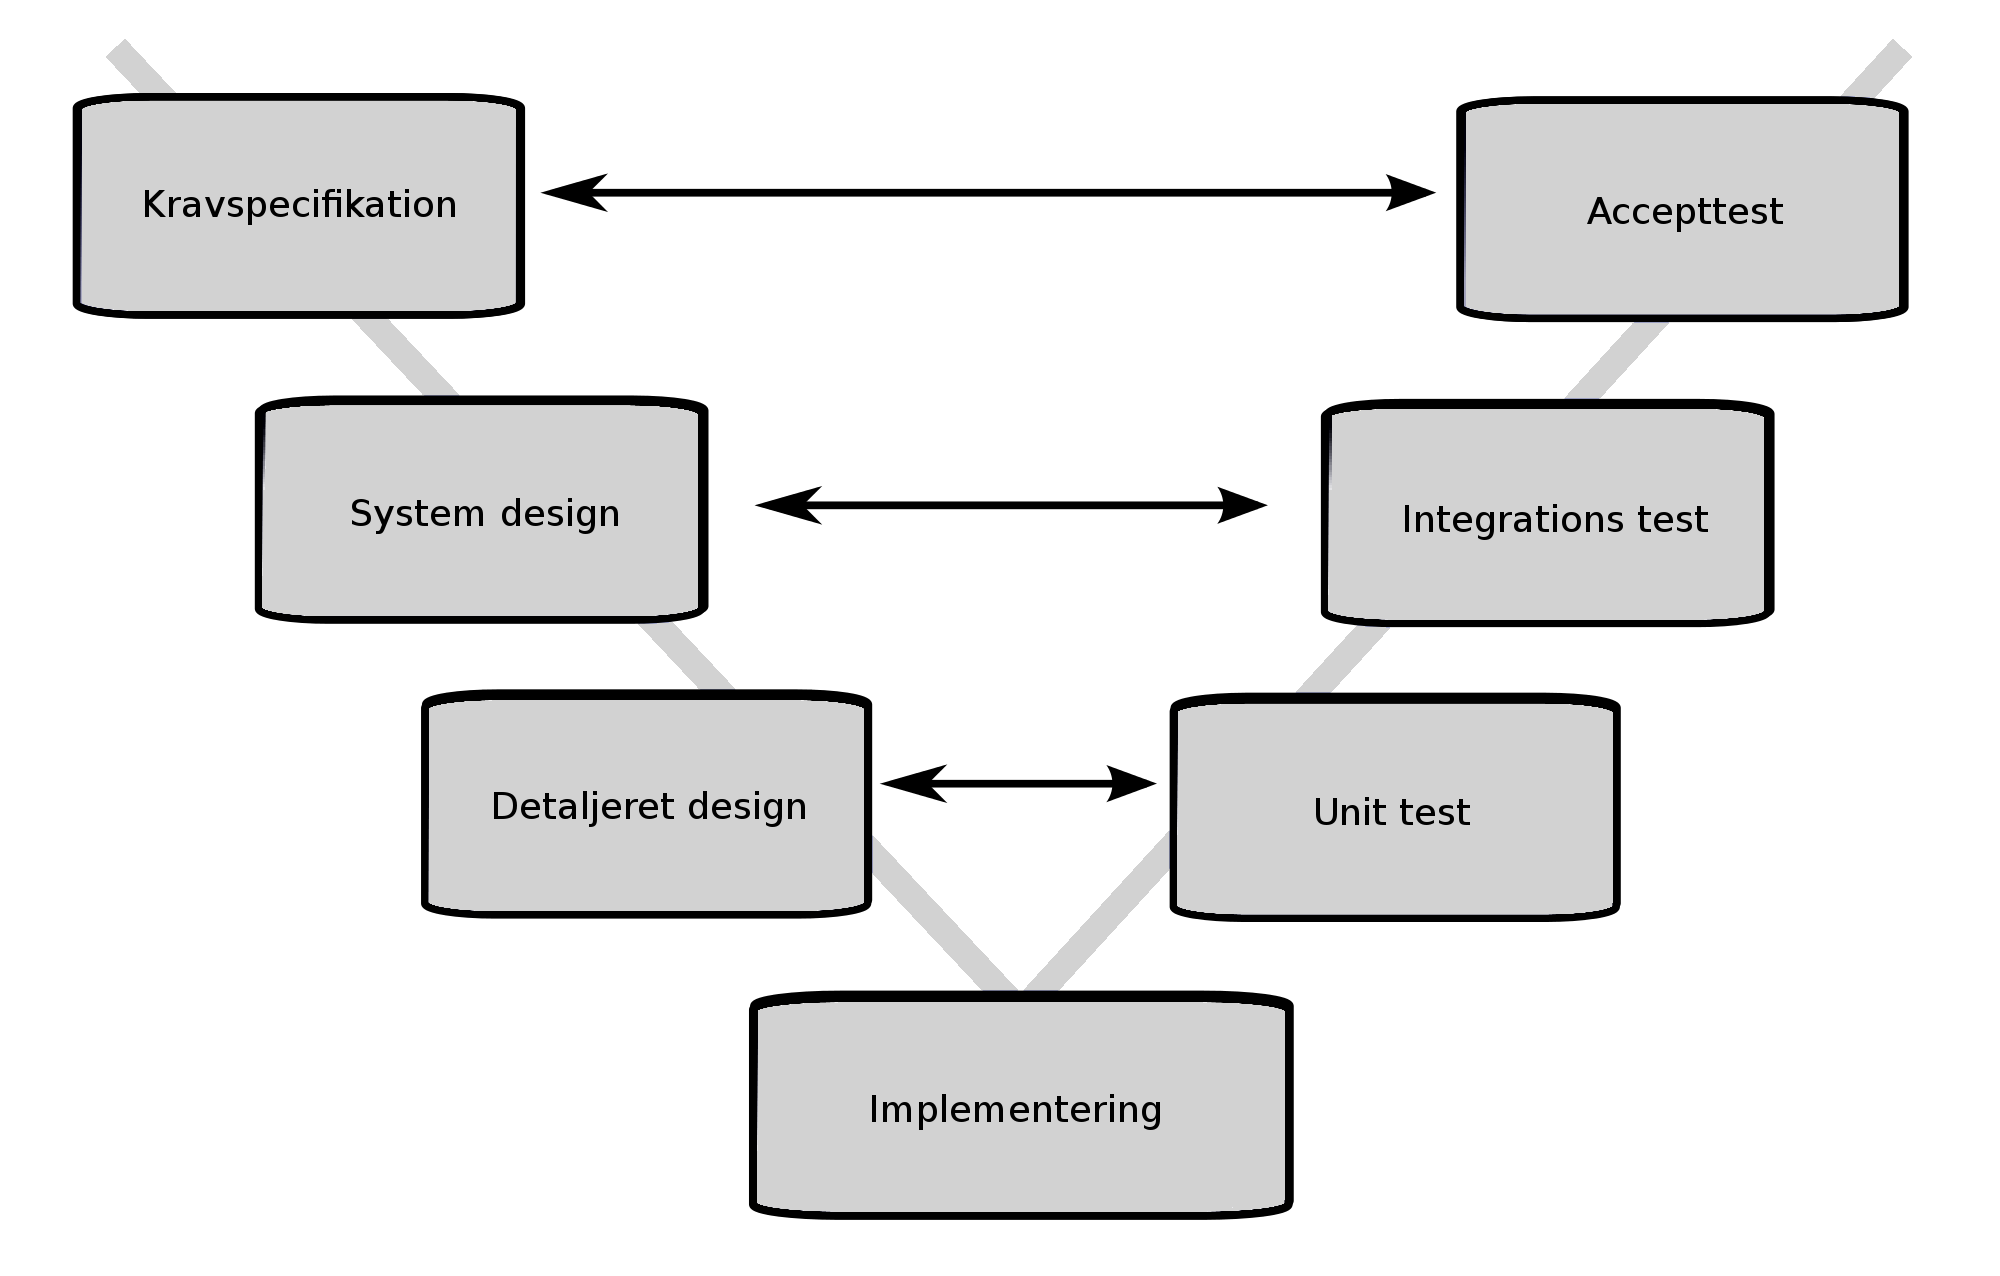
\includegraphics[width = \textwidth]{billeder/Vmodel.png}
	\caption{V-modellen}\label{fig:vmodel}
\end{figure}

\subsection{Review}
Review gruppen er beskrevet under afsnittet \ref{title:samarbejdspartnere}. Men review har også været en metode i udviklingsprocessen, i sammenfald med tidsplanen har reviewmøderne fungerede som deadline til hvornår bestemt mål skulle nåes i udviklingsprocessen. 

\subsection{3-lag modellen}
Denne metode bruges til at skabe struktur i \textit{Konditioneringsapparatets} software. 3-lags modellen sikre at der høj samhørighed og lav kobling mellem de tre lag. Inddelingen af konditioneringsapparatets software kan se system designet \fixme{Ref til system design} for mere information. 
\begin{figure}[H]
	\centering
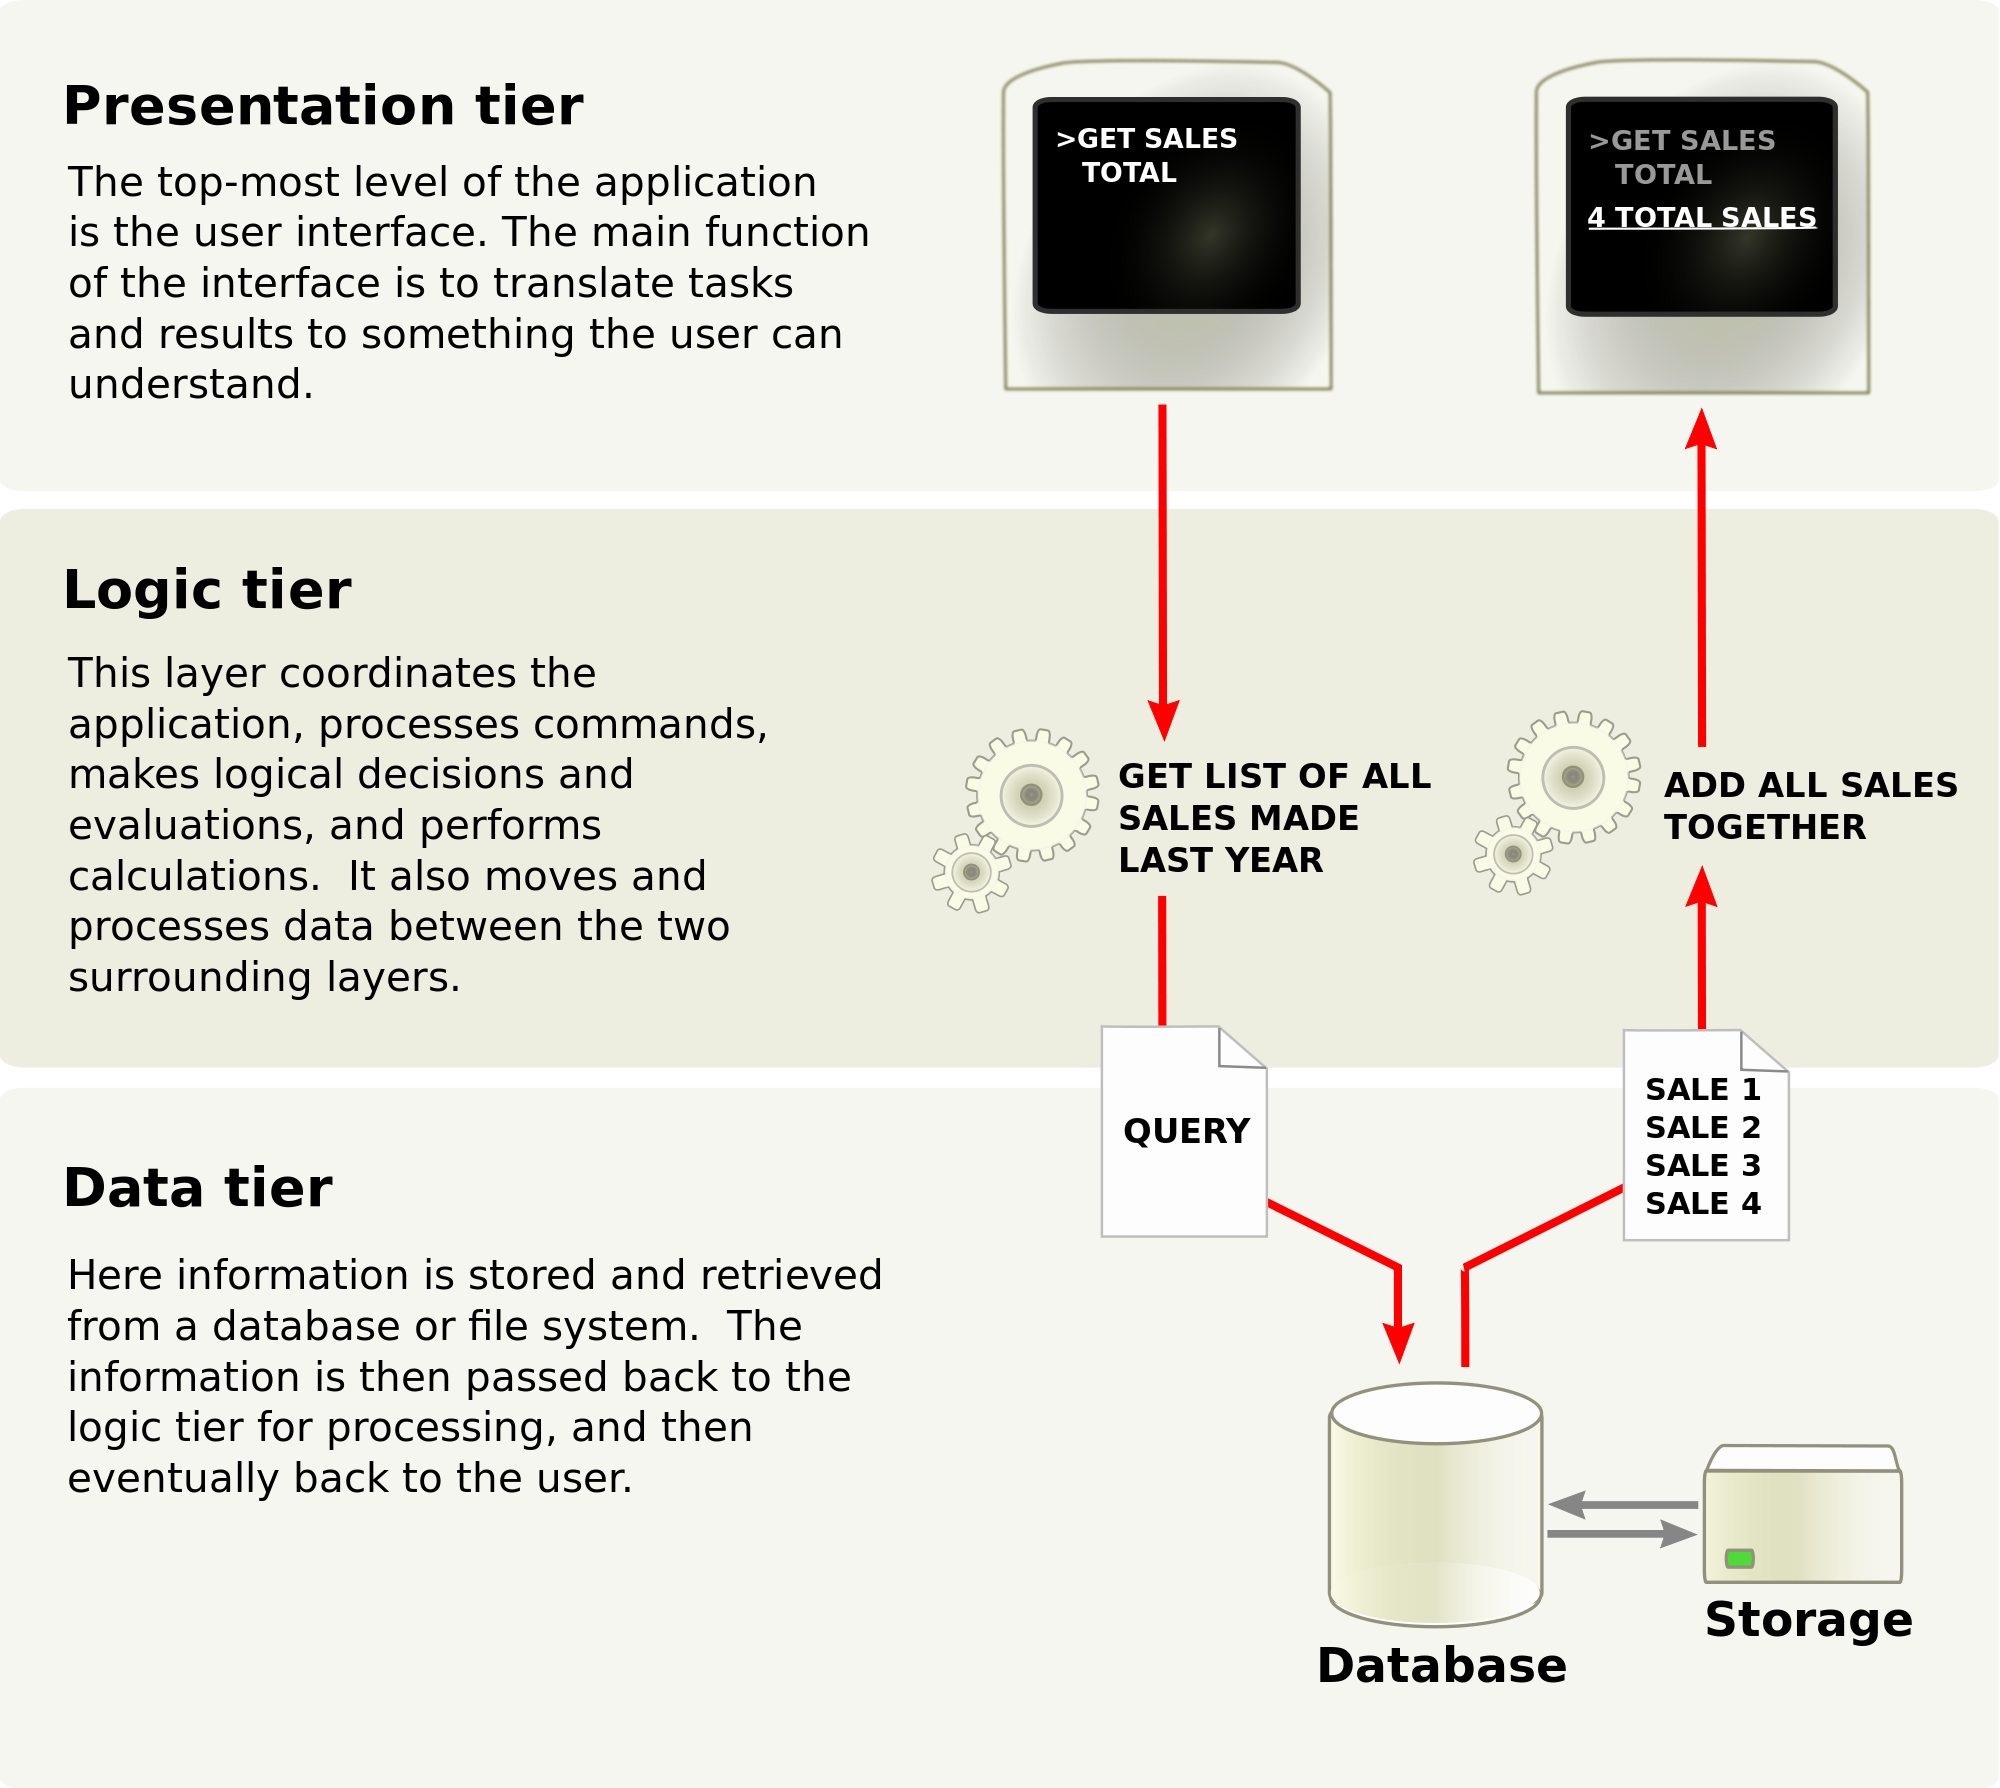
\includegraphics[width = 0.7\textwidth]{billeder/trelagsmodel.png}
\caption{Illustration af trelags-modellen med eksempel af typisk anvendse}\label{fig:3lagsmodel}
\end{figure}
\fixme{ref: til https://en.wikipedia.org/wiki/Multitier\_architecture}\\
De tre lag (Se figur \ref{fig:3lagsmodel}) er som følger: \\
\textit{GUI / Præsentations laget:} Dette lag håndterer præsentationen til bruger. Metoder, der tilhører dette lag, har til formål at skabe brugerfeedback. \\
\textit{Logik laget: } Her håndteres udregninger, data processering og evalueringen. Dette lag fungere ydermere som kommunikationens lag mellem data og præsentationslag. 
\\ \textit{Data laget: } Dette lag beskæftiger sig med data håndtering. Her håndteres kommunikation med hukommelse, eksterne databaser og andet udefrakommende data.

3-lags modellen sikre yderligere at software er logisk struktureret, har høj fleksibilitet og er nem at implementere. (\cite{RefWorks:31})
